\chapter{Identification of highly boosted W/Z$\rightarrow$\qqbarpr and H$\rightarrow$\bbbar}
\label{ch:vtagging}

\FIXME{Assume that I already introduced jet clustering algorithms in Section~\ref{sec:jets}. And I already introduce the signal topology in Section~\ref{ch:dibosonIntro}.}

Large-cone jets (see Section~\ref{sec:jets}), also referred to as ``fat jets'', are used to reconstruct the W jet, Z jet, and H jet candidates resulting after the hadronization of the two quarks from the decay of highly boosted W, Z, and Higgs boson, respectively. To discriminate against multijet backgrounds, the analyses exploit both the reconstructed jet mass, which is required to be close to the boson mass, and the jet substructure arising from the two jet cores that correspond to the two high-\pt decay quarks.\\

The techniques to identify jets arising from the merged decay products of a single V or Higgs boson is referred to as ``V tagging" or ``H tagging", respectively. It employes novel jet substructure algorithms, which are described in Section~\ref{sec:jetsubalgo}. The features of the V tagging algorithm are described in Section~\ref{sec:vtagging} and its performance in both data and simulation are discussed. 
%Discrepancies between data and simulation in the jet substructure observables used to identify the signal jets are studied through a measurement in a top quark enriched sample of data, as discussed in Section~\ref{sec:vtagging}.
Finally, in Section~\ref{sec:htagging}, a procedure tuned to the specific properties of the Higgs boson decay into a bottom quark-antiquark pair is presented.

%%%%%%%%%%%%%%%%%%%%%%%%%%%%%%%%%%%%%%%%%%%%%%%%%%%%%%%%%%%%%%%%%%%%%%%%%%%
\section{Jet substructure observables}
\label{sec:jetsubalgo}
%%%%%%%%%%%%%%%%%%%%%%%%%%%%%%%%%%%%%%%%%%%%%%%%%%%%%%%%%%%%%%%%%%%%%%%%%%%

\subsection{Pruned jet mass}
\label{subsec:pruning}

As the mass of the V or H boson is larger than the mass of a typical QCD jet, the jet mass is the primary observable that distinguishes a W jet from a QCD jet. The bulk of the W jet mass arises from the kinematics of the two jet cores that correspond to the two decay quarks. In contrast, the QCD jet mass arises mostly from large-angle and soft gluon radiation.
As a first step in exploring potential substructure, the jet constituents are subjected to a jet grooming algorithm that improves the resolution in the jet mass and reduces the effect of pileup~\cite{Chatrchyan:2013vbb,Khachatryan:2014vla}. The goal of jet grooming is to recluster the jet constituents, while applying additional requirements that eliminate soft, large-angle QCD radiation. This procedure shifts the jet mass of QCD jets to smaller values, while maintaining the mass for signal jets close to the boson mass. Furthermore, soft contributions from the underlying event and pileup, usually present in all jets, are removed.
Different jet grooming algorithms have been explored at CMS and their performance on jets in multijet processes has been studied in detail~\cite{Chatrchyan:2013vbb,Khachatryan:2014vla}. In this analysis, the \emph{jet pruning} algorithm~\cite{jetpruning1,Ellis:2009me} is used, as it provides the best discrimination against QCD background as discussed in Ref.~\cite{Chatrchyan:2013vbb,Khachatryan:2014vla}.

Jet pruning reclusters each large-cone jet starting from all its original constituents, through the implementation of the CA algorithm, but applying two additional conditions beyond those given in \FIXME{refer to the general jet clustering equation}. In particular, the softer of the two particles $i$ and $j$ to be merged is removed when the following conditions are met:

\begin{equation}
z_{ij} \equiv \frac{\mathrm{min}(p_{Ti} + p_{Tj})}{p_{Ti} + p_{Tj}} < z_{cut}\:\:,
\quad\quad\quad\quad
\Delta R_{ij} > D_{cut} \equiv \alpha\frac{m_j}{p_T}
\end{equation}

where $m_j$ and $p_T$ are the mass and transverse momentum of the originally-clustered jet, and $z_{cut}$ and $\alpha$ are parameters of the algorithm, chosen to be 0.1 and 0.5, respectively. In this particular choice of parameters, the algorithm removes the largest number of jet constituents, and can therefore be regarded as the most aggressive jet grooming technique. The resulting jet is the \emph{pruned jet}. The pruned jet mass, \mJ, is computed from the sum of the four-momenta of the constituents that survive the pruning; it is then corrected by the same factor used to correct the jet \pt (see Section~\ref{sec:jets}).
Figure~\ref{fig:mass_pr_a} illustrates the effect of pruning on AK8 jets: the \mJ spectrum of the W jet candidate from the decay of highly boosted and longitudinally polarized W bosons is shown together with the distribution in \mJ for the simulated background of W+jets. Dashed and solid lines correspond to the distributions before and after the application of the pruning algorithm, respectively. Fully merged jets reconstructed from the W boson decay generate a distinctive peak around the W boson mass, which is narrowed by the pruning, while background jets acquire a smaller mass on average, enhancing the discrimination. Figure~\ref{fig:mass_pr_b} compares the distributions in \mJ for W, Z and H jet candidates from the decay of highly boosted W, Z and Higgs bosons, respectively. The distribution in \mJ for the W+jets background is also shown. Not-full-merged signal jets give rise to a peak at low masses. 
%The \mJ distributions for W jets and QCD jets are shown in Fig.~\ref{fig:mass_pr} at generator level and reconstruction level with pileup. Comparing the generator level predictions for the \mJ of W jets with those at detector level with pileup, the widening of the peak due to detector resolution can be observed.

\begin{figure}[!htb]
\centering     %%% not \center
\subfigure[]{\label{fig:mass_pr_a}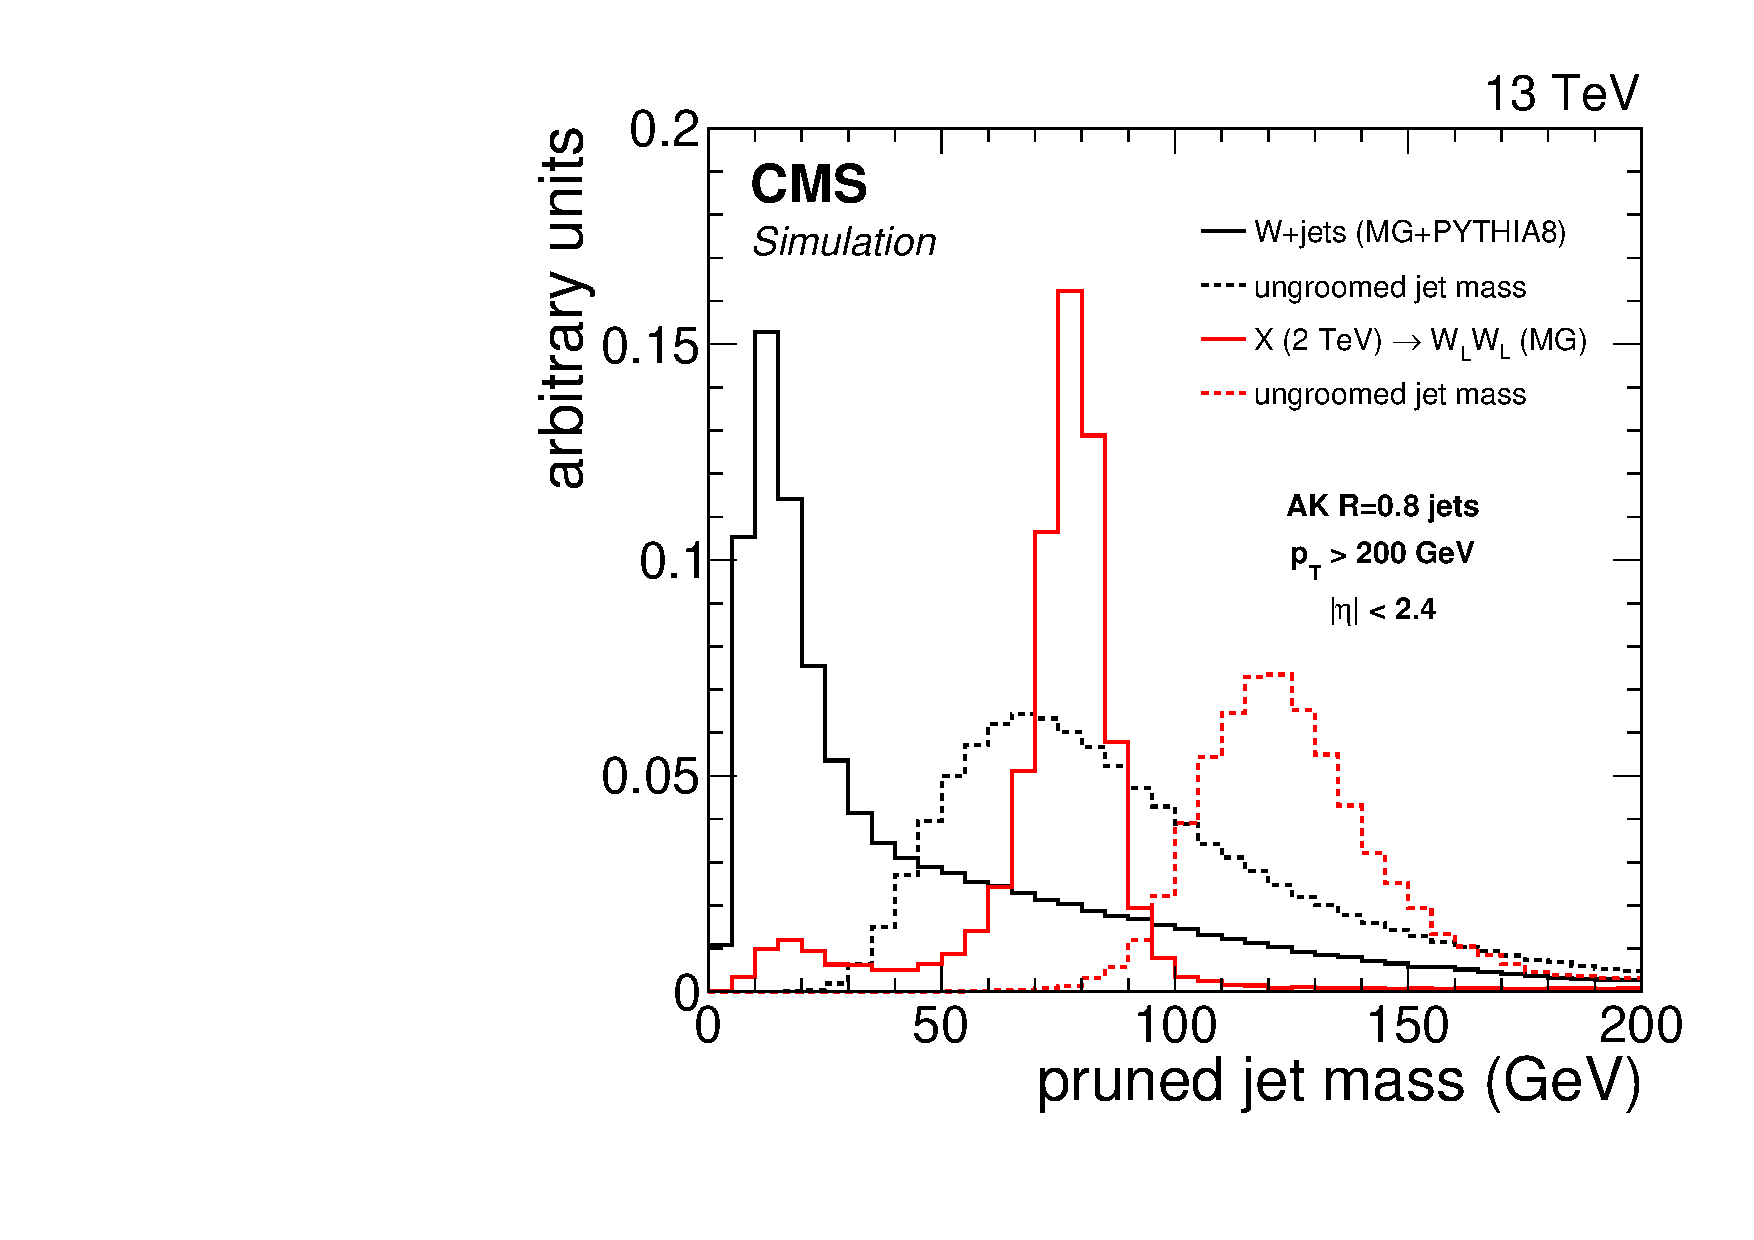
\includegraphics[width=0.45\textwidth]{\chseven/pruned-jet-mass.pdf}}
\subfigure[]{\label{fig:mass_pr_b}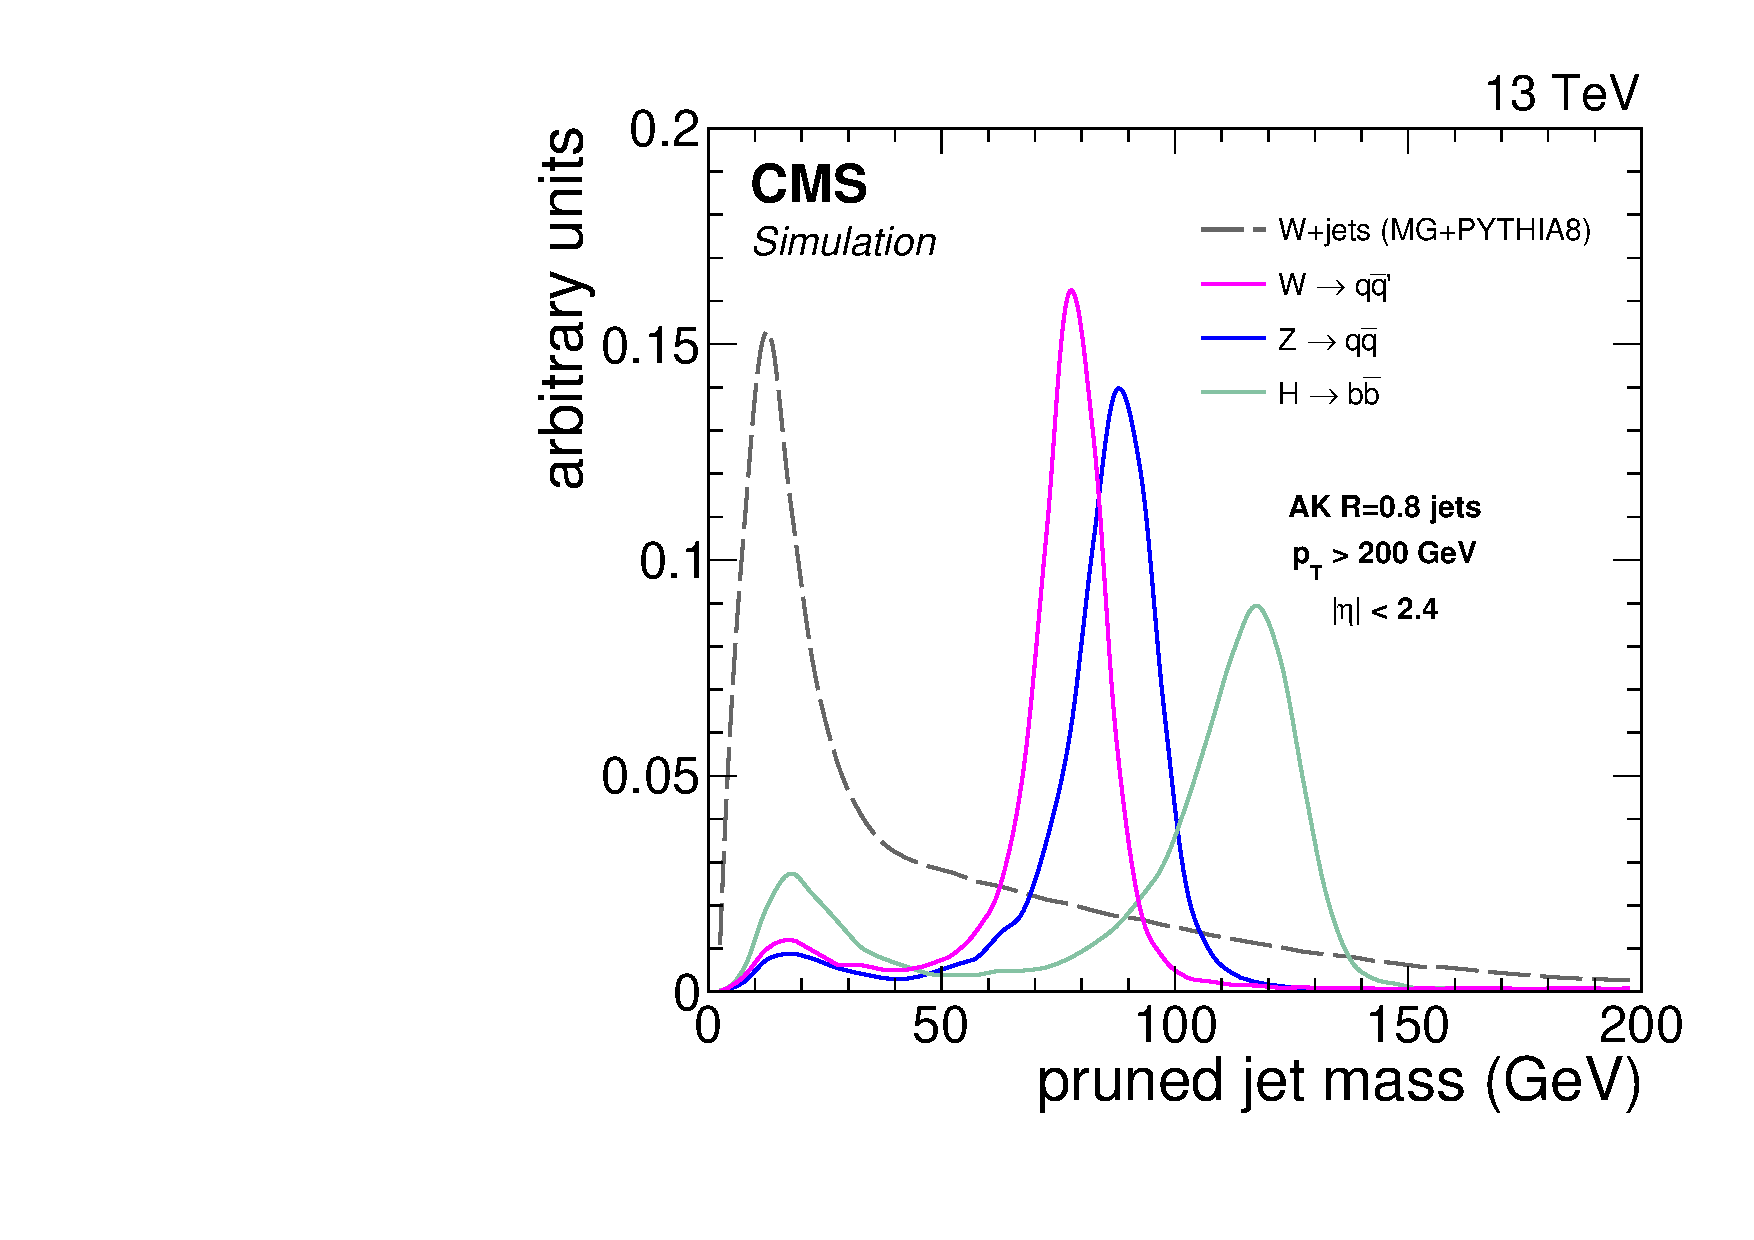
\includegraphics[width=0.45\textwidth]{\chseven/pruned-jet-mass-allsignals.pdf}}
\caption{(a) Distribution in pruned jet mass \mJ for simulated events of highly boosted W bosons and inclusive QCD jets expected in the W+jet topology. The ungroomed jet mass is shown as dotted lines to illustrate the effect of pruning. MG denotes the MADGRAPH generator. (b) Comparison of the distributions in \mJ for simulated events of highly boosted V and Higgs bosons.}
\label{fig:mass_pr}
\end{figure}
 
%In considering the kinematics of the substructure, two variables, $z$ and $\theta$, are particularly useful. For a recombination 1,2 $\rightarrow$ p, they are defined as:
%\begin{equation}
%z \equiv \mathrm{min}(p_{T1} + p_{T2})/p_{Tp}\:\:,
%\quad\quad\quad\quad
%\theta \equiv \Delta R_{12}
%\end{equation}
%To identify heavy particle decays reconstructed in a single jet, the interest is in recombinations that occur at large $\theta$, typically the final recombination. In general, small-$\theta$ recombinations are likely to represent the QCD showering of the decay products. Similarly, small-$z$, or soft, recombinations are typical for a QCD shower. Even the large-angle, but small-$z$, recombinations that can appear in jets from a heavy particle decay will be unlikely to yield an accurate representation of the decay: if a heavy particle decays such that one decay product has a much lower \pt relative to the others, the parent particle is unlikely to be accurately reconstructed.

%from JME-16-003: The softdrop algorithm is primarily aimed at separating W-jets from q/g-jets and does not fully reject contributions from underlying event and pileup. Therefore, a jet shape aware pileup suppressing algorithm needs to be applied in addition. We study softdrop in combination with the PUPPI algorithm 
%The pairwise merging scheme of recombination algorithms naturally gives substructure to a jet, which provides kinematic handles to determine whether the jet was produced by QCD alone or a heavy particle decay plus QCD.

\subsection{N-subjettiness}
\label{subsec:nsubj}

In addition to the pruned jet mass, additional information about the jet shape is used to discriminate the signal against jets from gluon and single-quark hadronization. This information can be obtained from the quantity called \emph{N-subjettiness}~\cite{Thaler:2010tr}. It takes advantage of the multi-body kinematics in the decay pattern of boosted hadronic objects, and it can be used to effectively ``count'' the number of subjets in a given jet. 

The N-subjettiness is a generalized jet shape observable which defines a measure, $\tau_N$, for a jet to have $N$ subjets. The constituents of the jet before the pruning procedure are reclustered using the $k_T$ algorithm (see Section~\ref{sec:jets}), until $N$ joint objects (subjets) remain in the iterative combination procedure of the algorithm. The observable $\tau_N$ is then defined as

\begin{equation}
\tau_N = \frac{1}{d_0} \sum_{k} p_{T,k}~\mathrm{min} \{\Delta R_{1,k},\Delta R_{2,k},\cdots,\Delta R_{N,k}\}
\end{equation}

where $k$ runs over the constituents of the jet, and the distances $\Delta R_{n,k}$ are calculated relative to the axis of the $n$th subjet. %We use a one step optimization of the exclusive kT axes to define the subjet axes.
The normalization factor $d_0$ is taken as

\begin{equation}
d_0 = \sum_{k} p_{T,k} R_{0}
\end{equation}

where $R_0$ is the characteristic jet radius used in the original jet clustering algorithm. The subjet axes are obtained by running the exclusive $k_T$ algorithm~\cite{Ellis:1993tq}, and reversing the last $N$ clustering steps. The variable $\tau_N$ quantifies to what degree the jet can be regarded as a jet composed of $N$ subjets. Jets with $\tau_N \approx 0$ have all their radiation aligned with the candidate subjet directions and therefore have $N$ (or fewer) subjets. Jets with $\tau_N \gg 0$ have a large fraction of their energy distributed away from the candidate subjet directions and therefore have at least $N+1$ subjets.
%The \tau_N$ observable has a small value if the jet is consistent with having N or fewer subjets, as almost every jet constituent will be close in ?R to its own true subjet.
%For discrimination between W jets with two subjets and QCD jets consistent with a single subjet, the ratio $\tau_2/\tau_1$ is particularly useful as it tends to smaller values for W jets.
The ratio between 2-subjettiness and 1-subjettiness, $\tau_{21} = \tau_{2}/\tau_{1}$, is found to be a powerful discriminant between jets originating from hadronic V decays and from gluon and single-quark hadronization. Jets from W or Z decays in signal events are characterized by lower values of $\tau_{21}$ relative to QCD background.
%We find that ?2/?1 is an effective discriminating variable to identify two-prong objects like boosted W, Z, and Higgs bosons.
Figure~\ref{fig:tau21} shows the $N$-subjettiness ratio $\tau_{21}$ distribution for W jets and QCD jets after requiring 60 $< \mJ <$ 100\GeV, and demonstrates its discrimination power after the pruned jet mass selection. %The distributions at detector level with pileup are shifted significantly compared to the generator level predictions, though the discrimination power is preserved. The shift is due equally to detector effects and pileup.

\begin{figure}[!htb]
 \begin{center}
  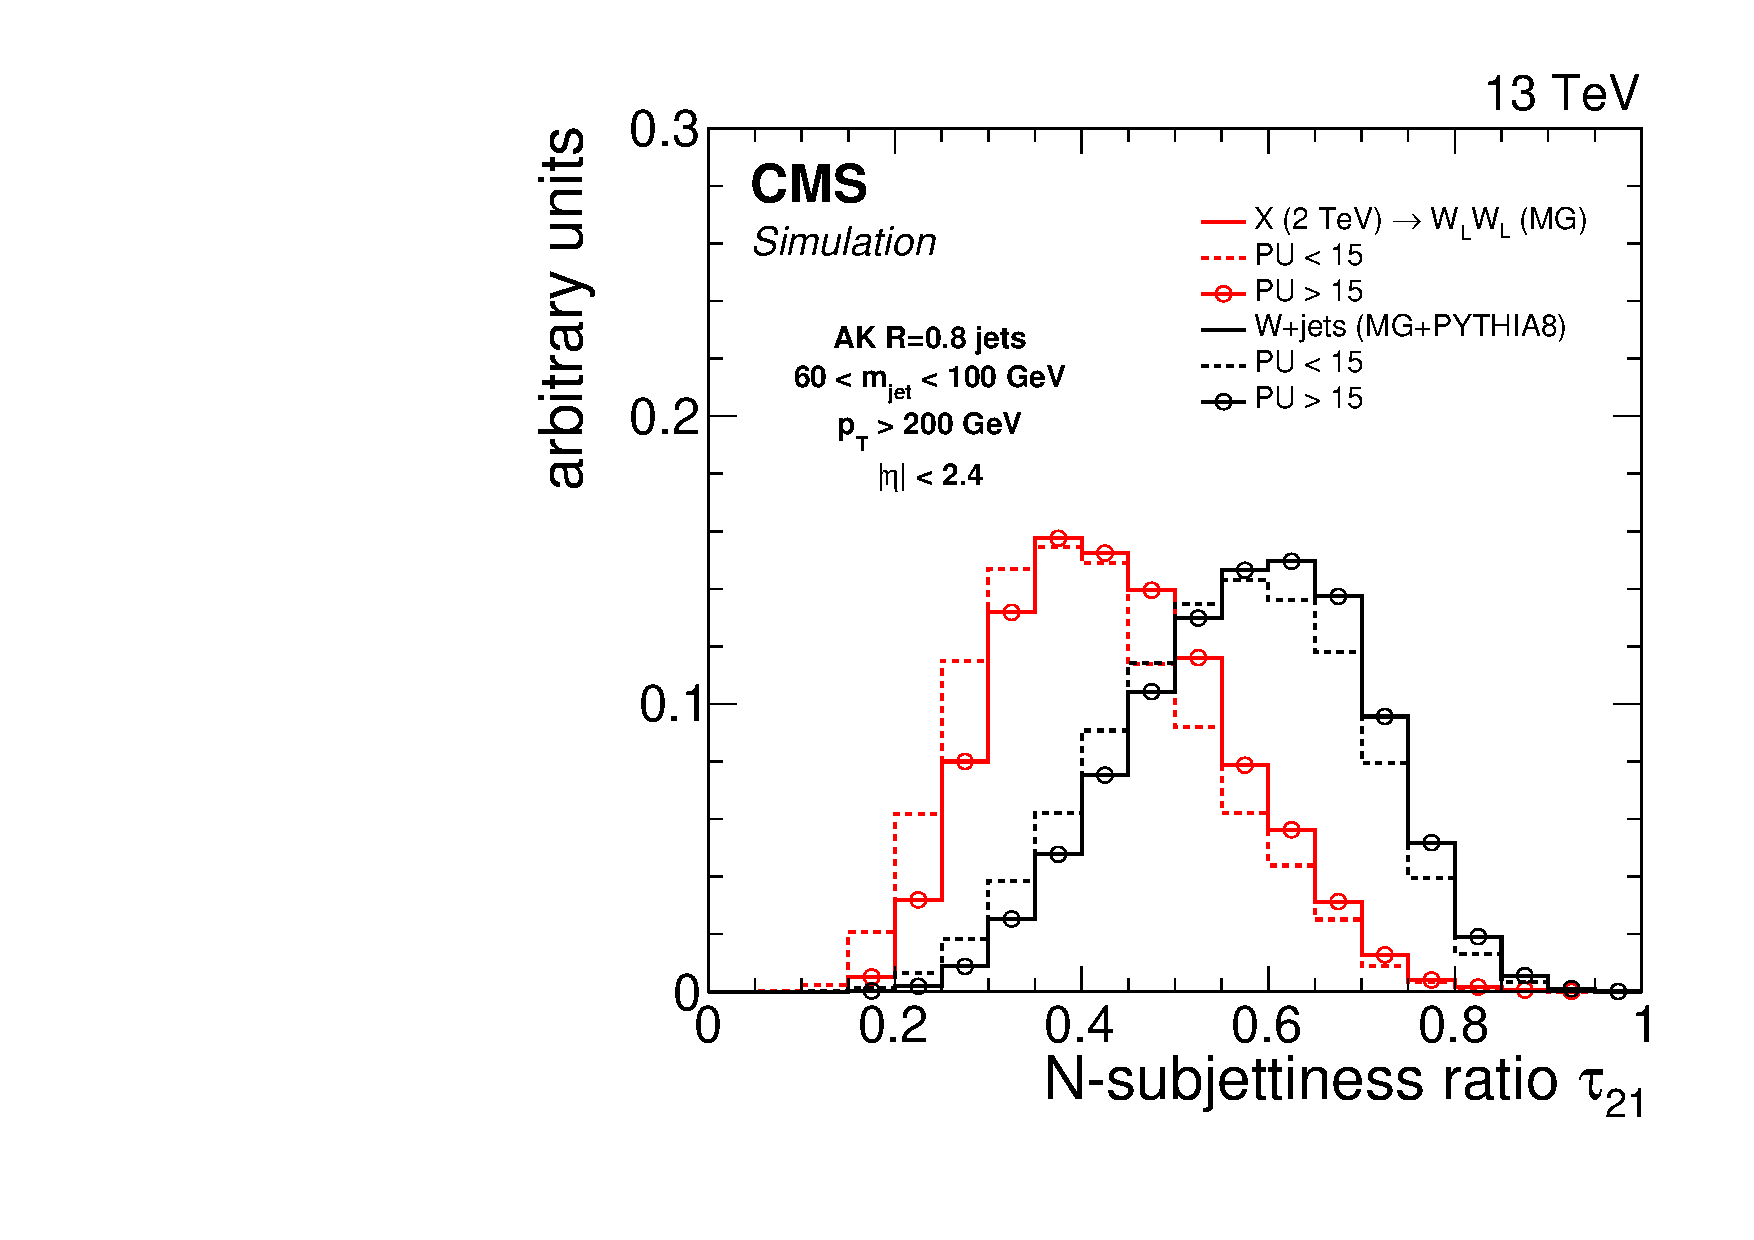
\includegraphics[width=0.5\textwidth]{\chseven/tau21.pdf}
 \end{center}
 \caption{\small Distribution in N-subjettiness ratio $\tau_{21}$ for simulated events of highly boosted and longitudinally polarized W bosons and inclusive QCD jets expected in the W+jet topology. The distributions are shown after a selection on the pruned jet mass requiring 60 $< \mJ <$ 100\GeV. MG denotes the MADGRAPH generator. The histograms are the expected distributions after full CMS simulation with pileup corresponding to an average number above and below 15 interactions.
 %Thick dashed lines represent the generator predictions without pileup interactions and without CMS detector simulation. 
 }
 \label{fig:tau21}
\end{figure}

%%%%%%%%%%%%%%%%%%%%%%%%%%%%%%%%%%%%%%%%%%%%%%%%%%%%%%%%%%%%%%%%%%%%%%%%%%%
\section{The V tagging algorithm}
\label{sec:vtagging}

The substructure techniques described in the previous section are employed for identifying, or ``tagging'', W and Z jets (``V jets''). The V tagging of the jets is obtained combining selections on both the pruned jet mass \mJ and N-subjettiness ratio \nsubj observables. %If the conditions are met the jet is referred to as ``V jets''. 

The selection criteria have been optimized in the context of searches for resonances decaying into diboson in the \lnujet and dijet final states~\cite{Khachatryan:2014gha,Khachatryan:2014hpa,CMS-PAS-EXO-15-002}. The optimization, based on simulation, aims at maximizing the analysis sensitivity and it leads to slightly different working points for each analysis. Typical signal efficiencies and mistagging rates of QCD jets obtained, respectively, from simulations and measurements for $\sqrt{s}$ = 8 and 13 TeV are summarized in Table~\ref{tab:vtagging}, for jets with \pt = 500\GeV.

\begin{table}[!htb]
\centering
\caption{Typical selection criteria for V tagging in 8 and 13 TeV analyses. The corresponding signal efficiency and mistagging rate of QCD jets are also reported for jets with \pt = 500\GeV.}
\begin{tabular}{c|c|c|c}
$\sqrt{s}$                     & V tagging selections      & signal efficiency          & mistagging rate\\
\hline
\hline
\multirow{2}{*}{8\TeV}  & 60 $< \mJ <$ 100\GeV  & \multirow{2}{*}{0.65}   & \multirow{2}{*}{0.04}\\
                                    & \nsubj $<$ 0.5                &                                    & \\
\hline
\multirow{2}{*}{13\TeV} & 65 $< \mJ <$ 105\GeV  & \multirow{2}{*}{0.55}   & \multirow{2}{*}{0.03}\\
                                     & \nsubj $<$ 0.45              &                                    & \\
\end{tabular}
\label{tab:vtagging}
\end{table}

The \lnujet analysis described in this work makes use of a looser \nsubj working point of 0.6 resulted from an optimization which takes into account signal efficiency and background rejection over a large jet \pt range .
In fact, this channel is characterized by a low background rate and a \nsubj selection which provides enhanced signal efficiency over the whole jet \pt range is therefore preferred. This working point corresponds to a signal efficiency of 65\% and a mistagging rate of 5\%.\\

%behaviour with pt of mjet
The V tagging performance at 8 TeV have been studied in detail in Ref.~\cite{Khachatryan:2014vla}. From simulation studies it is observed that the efficiency of the \mJ selection increases with \pt up to about 600\GeV since at higher \pt the showers from the W decay quarks are more likely to be reconstructed within a single large-cone jet. Above 600\GeV, the efficiency begins to decrease as a function of jet \pt, since at very large values the PF candidate reconstruction degrades in resolving the jet substructure and the pruning algorithm therefore removes too large a fraction of the jet mass. For Run II of the LHC, the particle flow reconstruction has been optimized by exploiting the full potential of the CMS ECAL granularity to resolve jet substructure and a constant efficiency is maintained up to at least \pt = 2.5\TeV~\cite{CMS-PAS-JME-14-002,JME-16-003}.

%behaviour with pt of tau21
The efficiency of the additional \nsubj selection also drops as a function of \pt. It is important to note that the same efficiency at an equivalent background rejection rate can be reached by adjusting the maximum \nsubj as a function of \pt. Therefore, a fixed working point will degrade the efficiency with increasing \pt. However, by shifting the working point, the same performance can be achieved. This possibility has not been explored yet in any of the searches which employ V tagging.

%behaviour with PU
The efficiency of the V tagging selection as a function of the number of reconstructed primary vertices (PV) has also been studied~\cite{JME-16-003}. It is observed that the efficiency of the \mJ selection is constant as a function of PV, whereas the additional \nsubj selection efficiency drops from 60\% at 0 PV to 40\% at 30 PV. However, the mistagging of the background also decreases with pileup for the same selection, yielding similar discrimination. Efficiency and mistagging rate are affected by pileup in the same way, since additional pileup shifts the \nsubj distribution towards higher values (towards background like) for both signal and background (see Fig.~\ref{fig:tau21}). Therefore, the same signal efficiency can be reached at the same background rejection rate for up to 30 reconstructed vertices by merely adjusting the \nsubj selection.
%at 8 TeV; the \mJ decreases by 6\% between 5 and 30 reconstructed vertices, whereas the additional ?2/?1 selection efficiency drops by 12% over the same range (somehow the drop was smaller). 

%polarization
An important factor that influences the V tagging performance is the polarization of the reconstructed V bosons. The pruned jet mass selection is less efficient for transversely polarized (V$_\mathrm{T}$) V bosons. This can be explained by a higher asymmetry in the \pt of the two quarks from the V$_\mathrm{T}$ boson decay, such that the pruning algorithm in a considerable fraction of events rejects the particles from the lower \pt quark and yields a much lower jet mass. In addition, the $\Delta R$ separation between the partons for pure longitudinally polarized (V$_\mathrm{L}$) V bosons is smaller on average than for V$_\mathrm{T}$ bosons and is more likely to be accepted by a large-cone jet. In the analysis presented in this work only V$_\mathrm{L}$  bosons are considered.\\

The \lnujet analysis described in this work relies on the modelling of the jet substructure variables \mJ and \nsubj in simulation. The data/simulation discrepancies in \mJ and \nsubj can bias the signal efficiency estimated from simulated samples. Therefore, the modelling of signal efficiency is cross-checked in a signal-free sample with jets having characteristics that are similar to those expected for a genuine signal~\cite{JME-16-003}. A pure sample of high-\pt W bosons, that decay to quarks and are reconstructed as a single large-cone jet, is obtained selecting \ttbar and single top quark events.

Scale factors for the \nsubj selection efficiency are extracted by estimating the selection efficiency on both data and simulation for the pure W jet signal. This is achieved by subtracting the background contribution.
%The pruned jet mass distribution is used to discriminate the pure W jet signal from background contributions.
The generated W boson in the \ttbar simulation provides a model of the contribution from the W jet peak in the pruned jet mass. The contribution from combinatorial background is derived from \ttbar simulation as well. This signal plus background model is fitted directly in the distributions of data and in their simulation.

The pruned jet mass distribution of events that pass and fail the \nsubj selection are fitted simultaneously to extract the selection efficiency on the pure W jet component. The ratio of data and simulation efficiencies are taken as the V tagging efficiency scale factor. Figure~\ref{fig:wtagging-13TeV} shows the fits obtained with 13\TeV data for the \nsubj $<$ 0.45 selection and similar results are obtained for the looser \nsubj $<$ 0.6 selection used in the \lnujet analysis presented in this work. 
%In this method, a simultaneous fit is performed to the jet mass distributions for the \nsubj selection to separate the W boson signal from the combinatorial components in the top quark enriched sample in both data and simulation as shown in Fig.~\ref{fig:wtagging-13TeV}.
The extracted scale factor for this selection is 1.01 $\pm$ 0.03 and it is used to correct the total signal efficiency and the VV background normalization predicted by the simulation.
The quoted uncertainty includes two systematic effects. One from the modelling of the nearby jets and \pt spectrum in \ttbar MC events, obtained by comparing the selection efficiency estimated from LO and NLO \ttbar simulation. %This uncertainty amounts to 3-17\%.
%The uncertainties quoted on the scale factor include different sources of systematic effects. The leading ones are due to the simulation of the \ttbar topology used to derive the data-to-simulation scale factors. An uncertainty is evaluated due to the modelling of the nearby jets and \pt spectrum in \ttbar MC events, by comparing the selection efficiency estimated from LO and NLO \ttbar simulation. This uncertainty amounts to 3-17\%.
%This is not our case! In addition, an uncertainty is calculated due to parton showering by comparing the selection efficiency estimated in \ttbar samples generated with POWHEG and interfaced with PYTHIA 8 with samples generated with POWHEG but interfaced with HERWIG++. This uncertainty amounts to 8.6\% and quantifies the discrepancy between the jet substructure modeling of PYTHIA8 and HERWIG++.
The other due to the choice of the models used to fit signal and background.
%Potential systematic effects due to the choice of the signal and background fit model have been
%evaluated, by comparing the estimated efficiency on simulated \ttbar samples with two different fit
%models. In the default model, the signal is purely modelled by a Gaussian peak, while the tails
%of the signal peak distribution are absorbed by the background fit model. In the alternative
%model, the signal is modelled by a Gaussian peak with tails including the non-peaking part of
%the W jets obtained from generator matched \ttbar simulation. The estimated efficiencies obtained
%with those two methods, corrected for the fraction of W jets in the tails, agree within 0.3-12\%.
The quadratic sum of these systematic uncertainties is found to be smaller than half of the statistical uncertainty on the scale factor. An additional uncertainty is calculated to account for the extrapolation of the scale factor from \ttbar events with an average jet \pt $\sim$ 200\GeV to higher momenta. This is estimated from the difference between PYTHIA8 and HERWIG++~\cite{Bahr:2008pv} showering models with a resulting factor of 
$4.53\% \times \displaystyle \ln(\pt/200\GeV)$.

The peak position in the W jet mass and its resolution are also extracted to obtain data-to-simulation corrections on the pruned jet mass listed in Tables~\ref{tab:Wmass8TeV} and~\ref{tab:Wmass13TeV}, as measured with 8 and 13\TeV data, respectively. The quoted uncertainties are statistical. The W jet mass scale in 13\TeV data is $\sim$1\% smaller than in simulation while its resolution is found to be larger by about 5\%. In 8\TeV data both the W jet mass scale and resolution in data are larger than that in simulation. In the simulation \mJ must therefore be shifted by 1.7 $\pm$ 0.6\% and $\sigma$ be enlarged by 11 $\pm$ 9\% to correct for the difference between data and simulation.
%To extract corrections to the jet mass scale and resolution, we use the mean $<$m$>$ and resolution
%\sigma value of the Gaussian component of the fitted function of the W bosons in the passed sample.

The mass peak position is slightly shifted relative to the W boson mass. The shift is found to be primarily due to extra radiation in the W jet from the nearby b quark, and additional effects are due to the presence of the extra energy deposited in the jet cone from pileup, underlying event, and initial-state radiation not completely removed in the jet pruning procedure.\\
%Additional requirements to reduce the combinatorial background from \ttbar improve the precision of the determined scale factor. Therefore, the angular distance $\Delta R$ between the W jet candidate and the closest b-tagged AK4 jet is required to be less than 2.0, which is typical for highly boosted top quark decays~\cite{toppaper}.
%The mass peak position is slightly shifted relative to the W boson mass because of the extra energy deposited in the jet cone from pileup, underlying event, and initial-state radiation not completely removed in the jet pruning procedure. For events with top quarks, additional energy contributions arise also from the possible presence of a b jet close to the W jet candidate. Additional requirements to reduce the combinatorial background from \ttbar improve the precision of the determined scale factor. Therefore, the angular distance $\Delta R$ between the W jet candidate and the closest b-tagged AK4 jet is required to be less than 2.0, which is typical for highly boosted top quark decays~\cite{toppaper}. 

Because the kinematic properties of W jets and Z jets are very similar, the same corrections are also used when the V jet is assumed to arise from a Z boson.

\begin{figure}[!htb]
\centering     %%% not \center
\subfigure[]{\label{fig:wtagging-13TeV_a}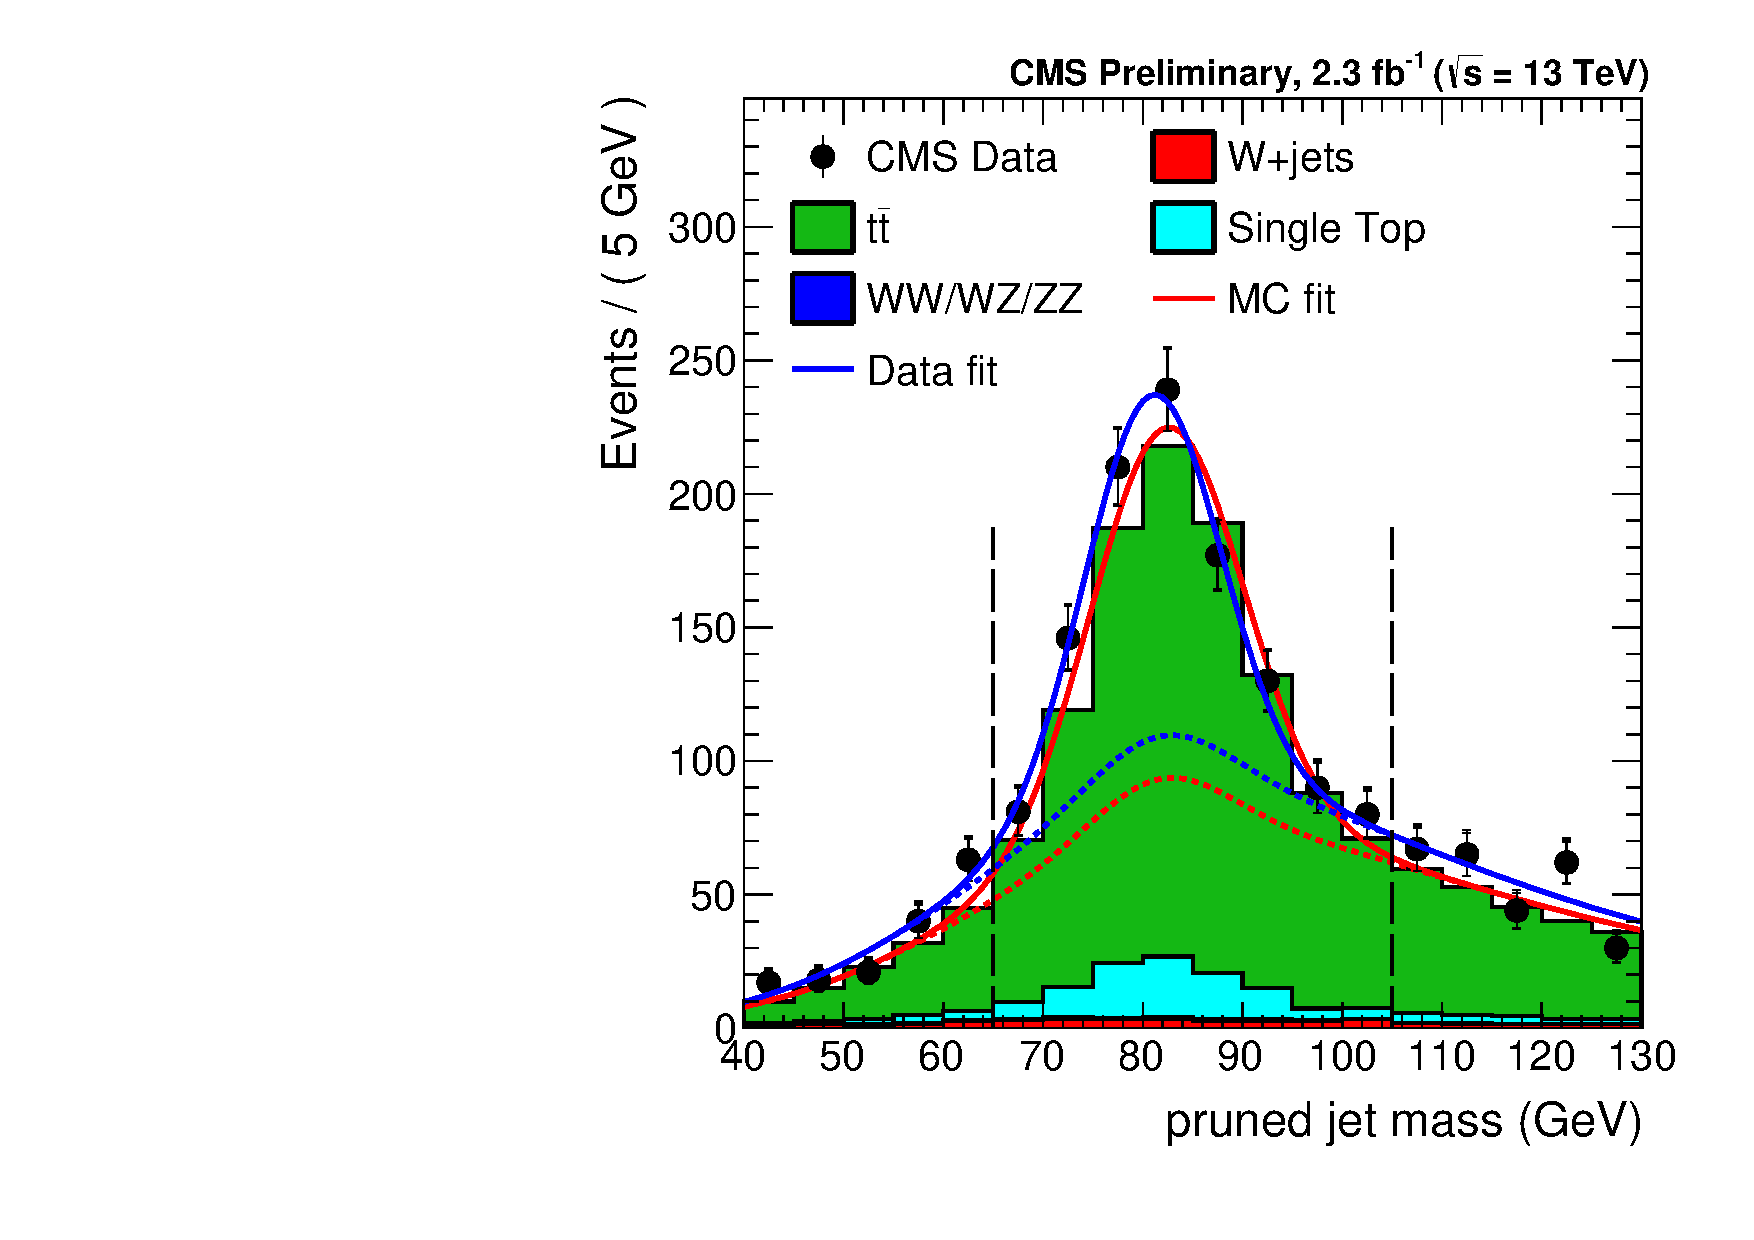
\includegraphics[width=0.45\textwidth]{\chseven/JME-16-003_HP0v45powheg_76X_em_pTbin_200_5000.pdf}}
\subfigure[]{ \label{fig:wtagging-13TeV_b}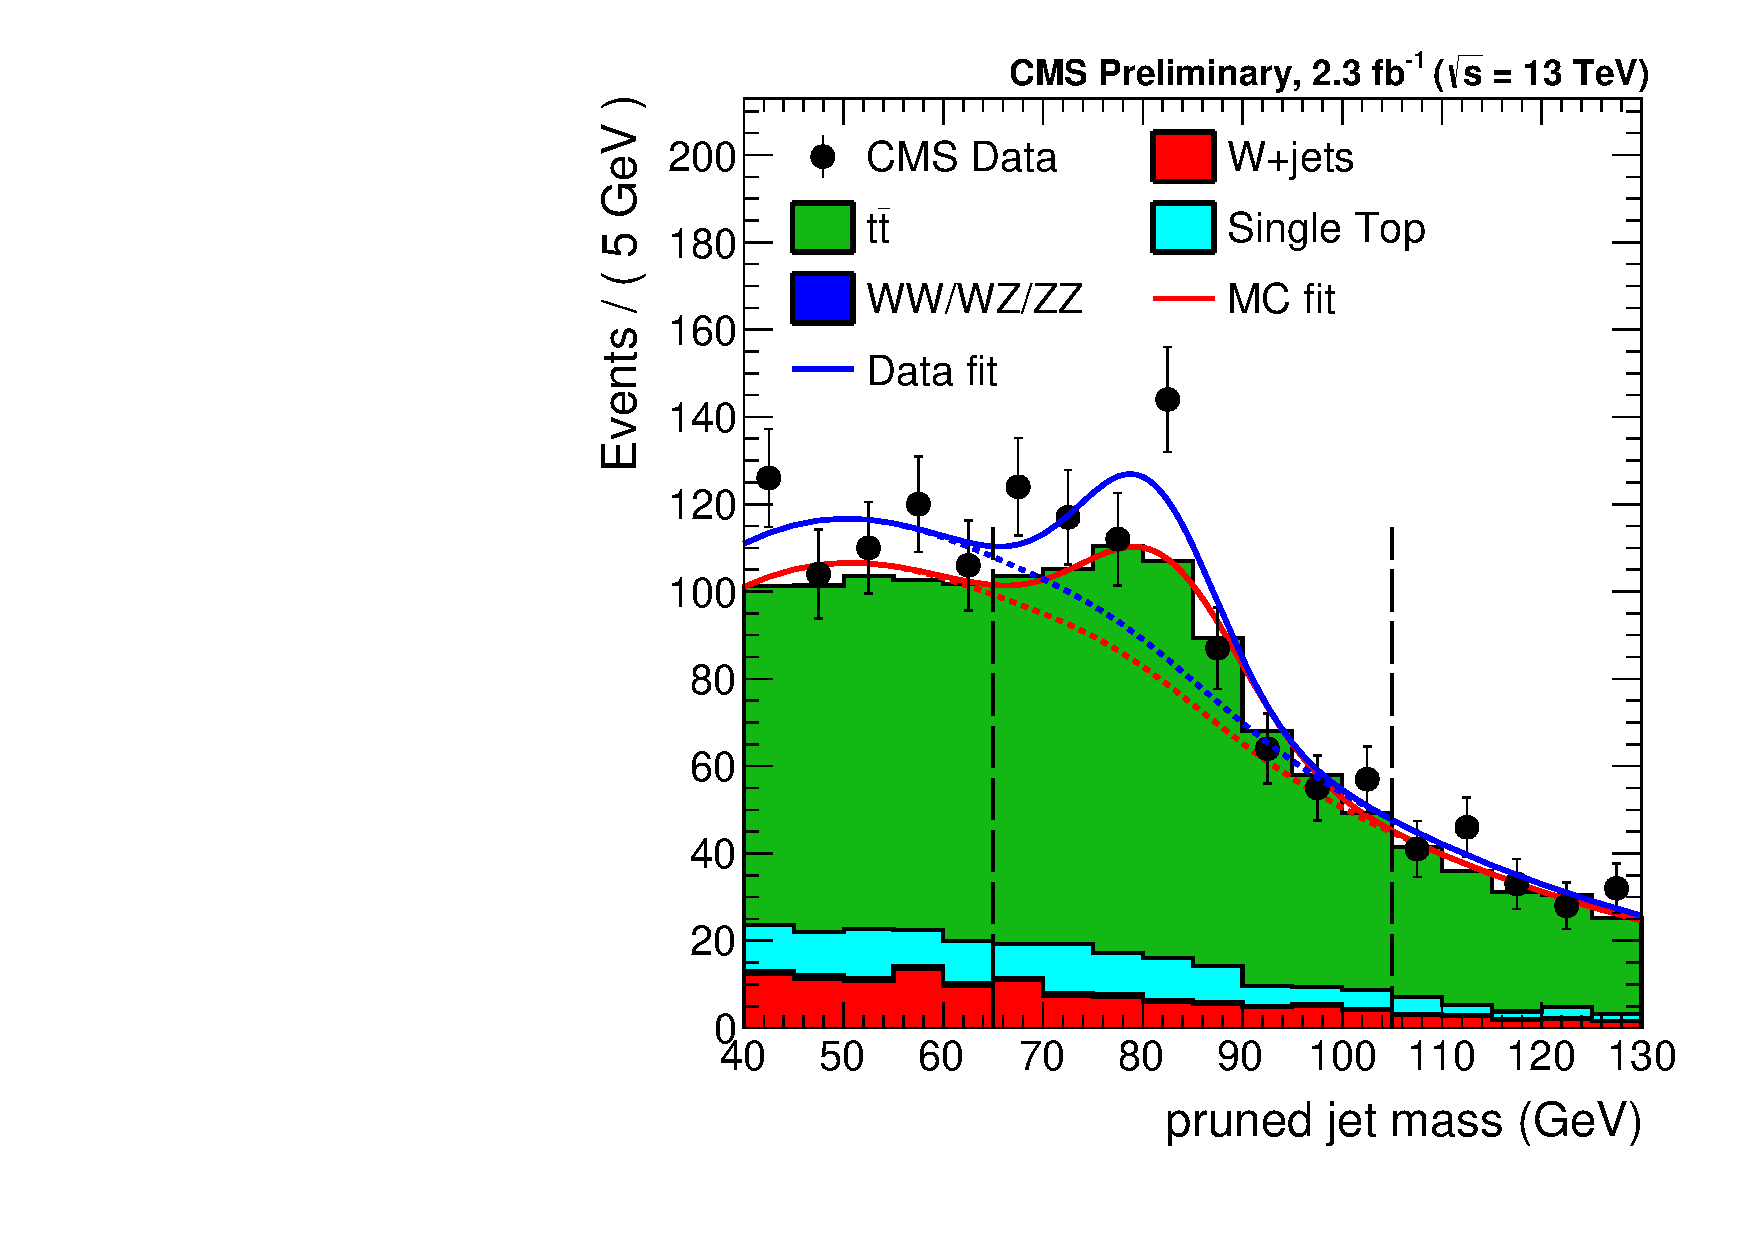
\includegraphics[width=0.45\textwidth]{\chseven/JME-16-003_HP0v45powheg_76X_em_fail_pTbin_200_5000.pdf}}
 \caption{Distribution in pruned jet mass for events that (a) pass and (b) fthe \nsubj $<$ 0.45 selection in the \ttbar control sample. The result of the fit to data and simulation are shown, respectively, by the solid and long-dashed line and the background components of the fit are shown as dashed- dotted and short-dashed line~\cite{JME-16-003}.}
 \label{fig:wtagging-13TeV}
\end{figure}

\begin{table}[!htb]
   \centering
   \caption{W jet mass peak position and resolution, as extracted from top quark enriched sample in 8\TeV data and from simulation, after applying the $\nsubj < 0.5$ selection~\cite{Khachatryan:2014vla}.}
   \begin{tabular}{lcc}
   \hline
   $\nsubj < 0.45$ & \mJ{} [\GeV] & Standard deviation~[\GeV]\\
   \hline
   Data          & 84.1 $\pm$ 0.4 & 8.4 $\pm$ 0.6\\
   Simulation & 82.7 $\pm$ 0.3 & 7.6 $\pm$ 0.4\\
   \hline
   \end{tabular}
   \label{tab:Wmass13TeV}
\end{table}

\begin{table}[!htb]
   \centering
   \caption{W jet mass peak position and resolution, as extracted from top quark enriched sample in 13\TeV data and from simulation, after applying the $\nsubj < 0.45$ selection~\cite{JME-16-003}.}
   \begin{tabular}{lcc}
   \hline
    $\nsubj < 0.5$ & \mJ{} [\GeV] & Standard deviation~[\GeV]\\
   \hline
   Data          & \WMASSDATAWPT & \WRESDATAWPT\\
   Simulation & \WMASSMCWPT    & \WRESMCWPT\\
   \hline
   \end{tabular}
   \label{tab:Wmass8TeV}
\end{table}

%%%%%%%quark/gluon composition
%The composition of the QCD background also influences the discrimination of the jet substructure variables, since the properties of quark- and gluon-initiated jets differ. For example, gluon jets tend to have a larger jet mass than quark jets and therefore fewer gluon jets are rejected by the pruned jet mass selection. On the contrary, the \nsubj discriminator rejects more gluon jets than quark jets and for these reasons a similar performance for quarks and gluons is achieved for a given \nsubj working point.
%%%%%%%%%data/MC comparison
%The W+jet and dijet events are compared in respective jet \pt bins of 250?350 \GeV and 400?600 \GeV, and with jets in the \ttbar sample with \pt $>$ 200\GeV. Simulation with different parton shower models of PYTHIA 6, PYTHIA 8 and HERWIG++ are also compared.
%A comparison of the distribution in the jet substructure observables between simulation and data have been performed in inclusive dijet, W+jet and \ttbar samples. In fact, the dijet and W+jet samples probe the V tagging variables using QCD jets, while a description of V jets can be obtained from a pure sample of real merged W bosons in high \pt lepton+jets \ttbar events. A good agreement is found between data and simulation for the \mJ distributions in dijet and W+jets samples, but HERWIG++ agrees better than PYTHIA 6, and PYTHIA 8 shows best agreement. The \nsubj variable is also found to agree better with HERWIG++ and best with PYTHIA 8.
%For \ttbar, POWHEG interfaced with PYTHIA 6 provides a better description than MC@NLO interfaced with HERWIG++.
%%%%%%%about the mistag rate
%A dijet sample is used to measure the rate of false positive W tags, or mistags. The mistagging rate is measured in data and compared to simulation
%The mistagging rate of only the mjet requirement in data is well reproduced by HERWIG++ and PYTHIA 8, while MADGRAPH+PYTHIA 6 underestimates it. When both the mjet and ?2/?1 requirements are applied, the mistagging rate in data is reproduced better by PYTHIA 8 than by MADGRAPH+PYTHIA 6 and HERWIG++. The pT dependence in data is well reproduced by all generators. The PU dependence is well reproduced by the simulation.

%\begin{figure}[h]
% \begin{center}
%  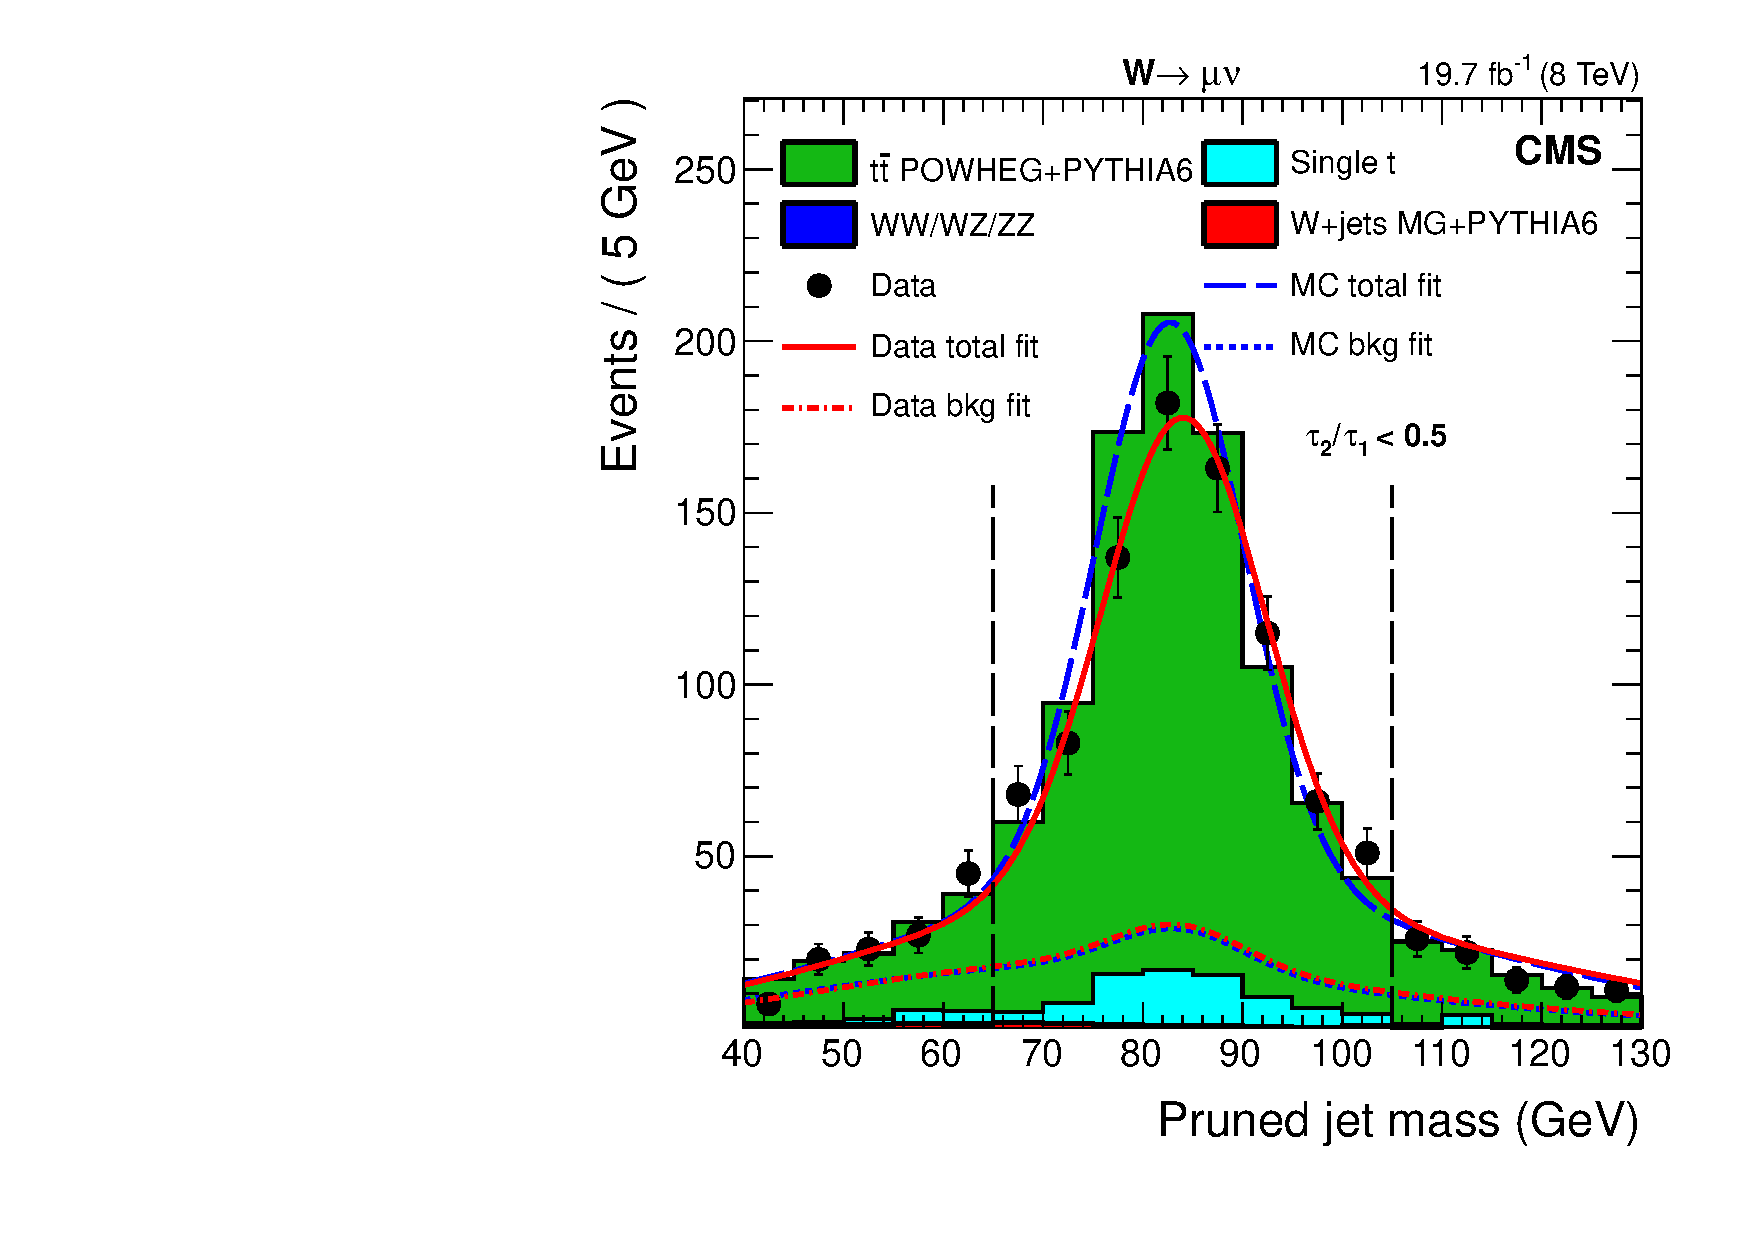
\includegraphics[width=0.48\textwidth]{\chseven/JME-13-006_control_HP_mu.pdf}
% 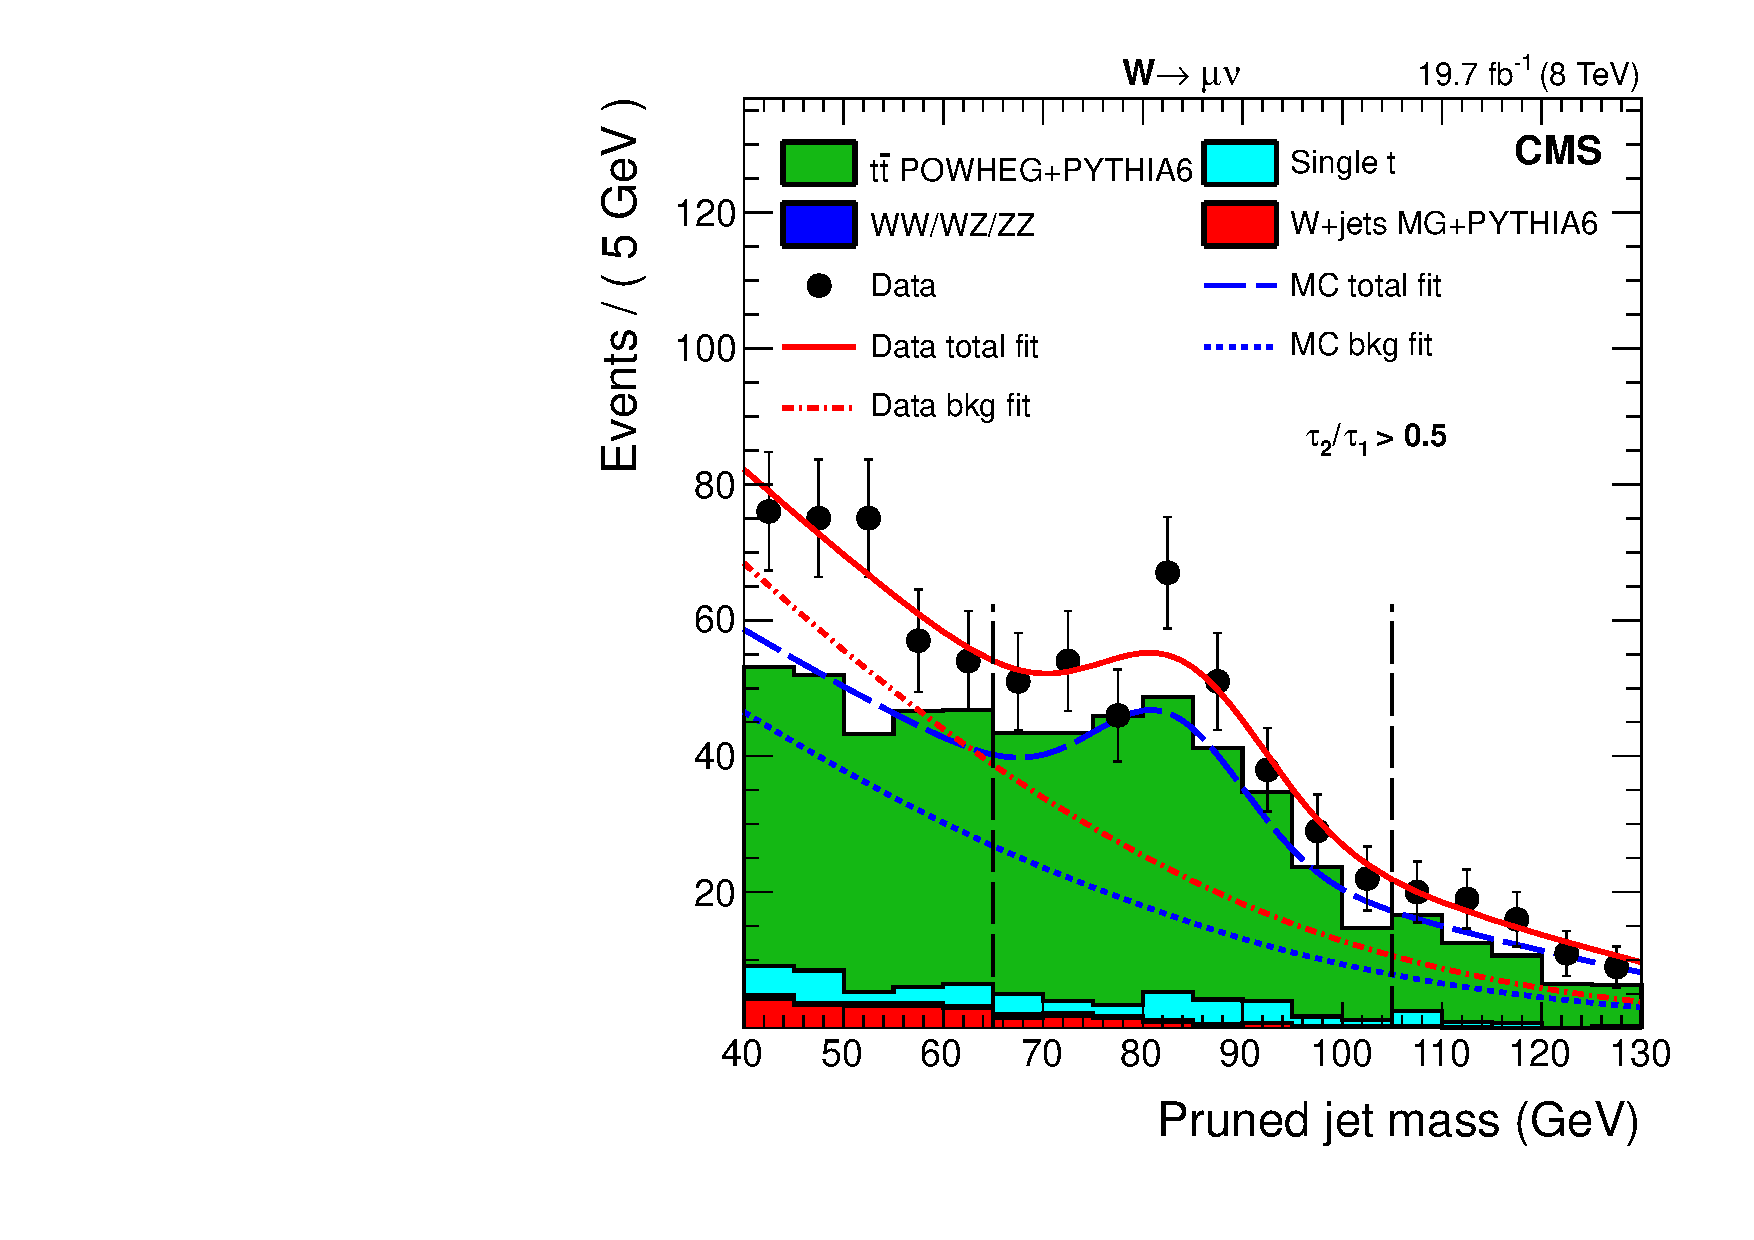
\includegraphics[width=0.48\textwidth]{\chseven/JME-13-006_control_HP_mu_fail.pdf}
%\end{center}
%\caption{W-tagging at 8 TeV (mu)~\cite{Khachatryan:2014vla}.}
%\label{fig:wtagging-8TeV}
%\end{figure}

%\begin{table}[htbp]
%   \centering
%   \topcaption{Data-to-simulation scale factors for the efficiency of the \nsubj selection used in the analyses, as extracted from top quark enriched data and from simulation.}
%   \begin{tabular}{lc}
%   \hline
%   \nsubj{} selection & Efficiency scale factor\\
%   \hline
%   $\nsubj < 0.45$              & \SFWTAGHPWPT \\
%   $0.45 < \nsubj < 0.75$   & \SFWTAGLPWPT \\
%   \hline
%   $\nsubj < 0.6$                & \SFWTAGHPWPL \\
%   \hline
%   \end{tabular}
%   \label{tab:WtaggingScaleFactors}
%\end{table}

%%%%%%%%%%%%%%%%%%%%%%%%%%%%%%%%%%%%%%%%%%%%%%%%%%%%%%%%%%%%%%%%%%%%%%%%%%%
\section{The H tagging algorithm}
\label{sec:htagging}

%introduction: say that a efficient higgs tagger is obtained exploiting both jet substructure and btagging
As discussed in the previous sections boosted V bosons are reconstructed using jet substructure methods
through the V tagging algorithm, providing large discrimination against multijet backgrounds.
However, if one or more of the decay products is a b quark, adding b jet identification (see Section~\ref{sec:jets}) together
with jet substructure information can significantly improve the sensitivity of these methods.
%In the previous sections the techniques deployed to reconstruct highly boosted V boson has been discussed.
%Boosted topologies are usually reconstructed and interpreted using the jet substructure methods such as top- and W/Z-tagging algorithms. 
%In the following we present methods of applying b tagging in boosted topologies along with a validation and measurement of the performance. 
%Several phenomenological studies have explored H $\rightarrow$ bb tagging algorithms (or ``H tagging'') using jet substructure, though ultimately the optimal
%performance comes from using both the substructure information of the fat jet and the track and vertex information related to the b hadron lifetime. 
%The approach presented here exploits both the jet substructure and the b tagging information aiming to identify the two b hadrons from the bb pair within the same fat jet.

%about the higgs tagger: subjet + fatjet btagging
Two different approaches to identify boosted H $\to$ \bbbar candidates have been explored
and used at CMS~\cite{CMS:BTV13001}:

\begin{itemize}
\item application of b tagging to the fat jet (``fat jet b tagging'')
\item application of b tagging to the subjets reconstructed within the fat jet (``subjets b tagging'')
\end{itemize}

Both approaches are based on the standard b tagging algorithms which take advantage of the tracking and vertexing information and are designed to identify jets from single b quarks.
%In the first approach the standard b tagging algorithms are applied to the fat jet but with the track and vertex association criteria relaxed due to a larger jet cone size, while in the second approach the subjets are first defined and then the standard b tagging is applied to each of the subjets. The performance of the fat jet b tagging is inherently limited by the fact that the algorithm is not designed to identify signal jets containing two b quarks.  On the other hand, the subjet b tagging, with its focus on individual subjets, does not fully profit from the global properties of the fat jets containing two b hadrons.  The two approaches are therefore complementary to an extent. The fat jet b tagging performs better in the high efficiency regime mostly relying on the presence of displaced tracks, while the subjet b tagging performs better in the high purity regime relying heavily on the reconstruction of secondary vertices associated to the subjets. Furthermore, at high \pt the subjets start to overlap causing the standard b tagging techniques to break down due to double-counting of tracks and secondary vertices when computing the subjet b-tag discriminants.  In Run I the subjet b tagging was mainly used at CMS to identify boosted H $\rightarrow$ bb candidates. While this approach is successful, its complementarity with the fat jet b tagging is a clear indication that further improvements can be achieved.
The CMS b tagging procedure starts with an association of tracks to jets, based on the angular distance between the tracks and the jet axis. 
The default b tagging algorithms use the selection $\Delta R < 0.3$.  However, when applying this to a large-cone jet of size R = 0.8, 
the criteria is suboptimal. Hence, to apply b tagging to fat jets, this angular distance is enlarged to $\Delta R < 0.8$. 
For the application of b tagging to subjets, the angular distance remains at the default value of $\Delta R < 0.3$.\\

The H tagging technique starts requiring that the pruned jet mass of the H jet candidate lies in a window around the Higgs boson mass (see Figure~\ref{fig:mass_pr_b}),
as this requirement rejects a large fraction of QCD background as demonstrated in the previous sections.
The subjets are then obtained by reversing the last step of the pruning recombination algorithm described in Section~\ref{subsec:pruning}.
In addition to the jet mass requirement, the b tagging is applied either to the whole fat jet or to the two subjets, where both subjets are required
to pass the same selection on the CSV discriminator. The b tagging efficiency and misidentification probability of QCD jets after applying the selection 75 $<$ \mJ $<$ 135\GeV is shown in Fig.~\ref{fig:htagging8TeV}.
The subjet b tagging outperforms the fat jet tagging for most of the phase space.
%A requirement on the pruned jet mass [26], 75 $<$ \mJ $<$ 135\GeV, is used, which rejects a large fraction of QCD background.

\begin{figure}[!htb]
\centering     %%% not \center
\subfigure[]{\label{fig:htagging8TeV_a}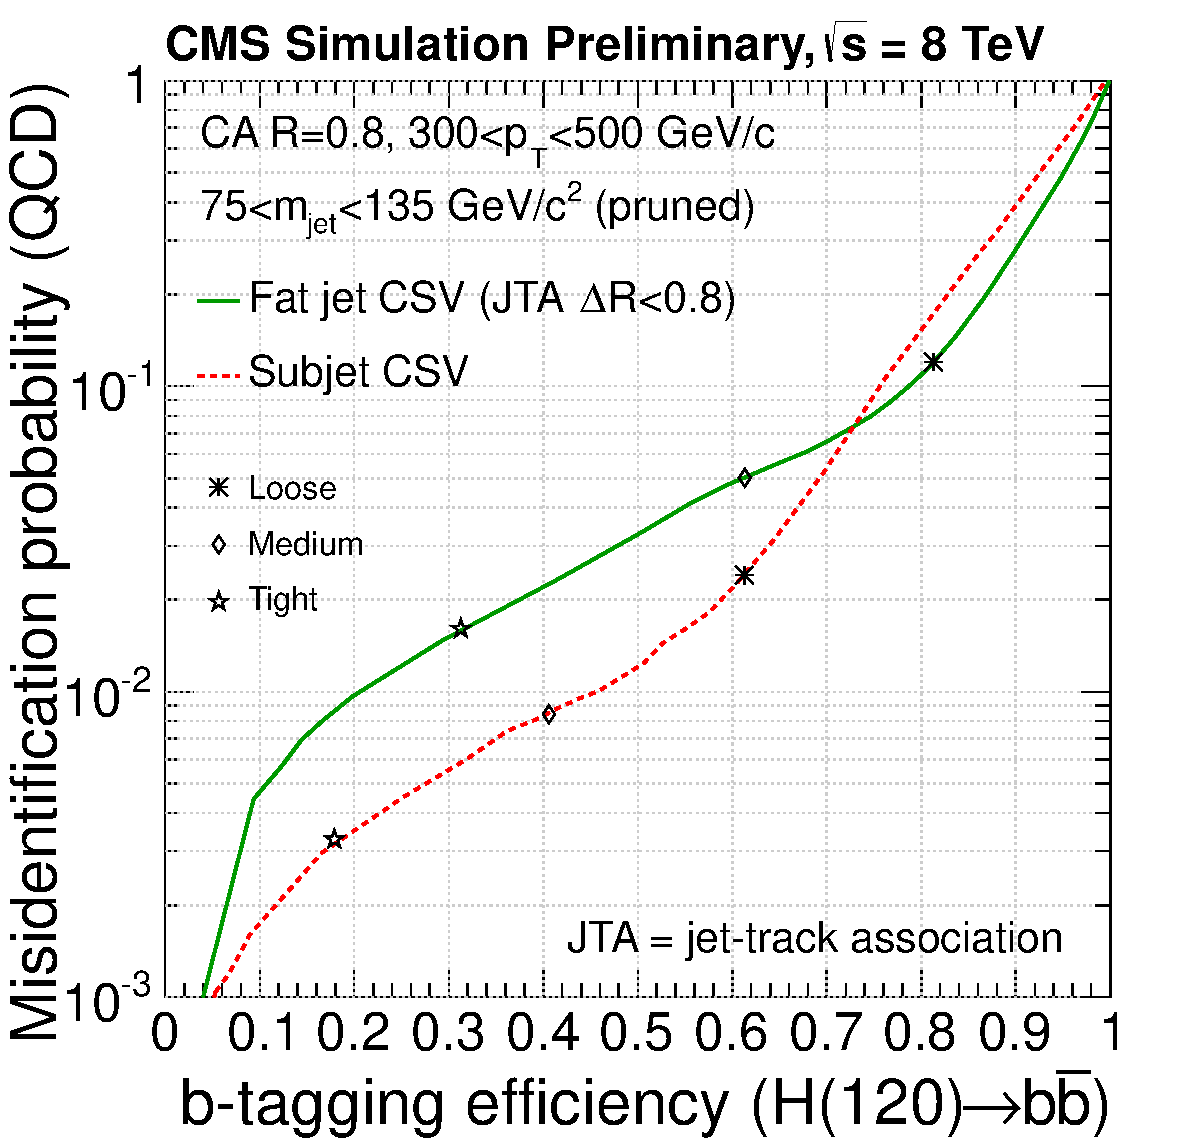
\includegraphics[width=0.45\textwidth]{\chseven/BTV-13-001_Figure_022-a.pdf}}
\subfigure[]{\label{fig:htagging8TeV_b}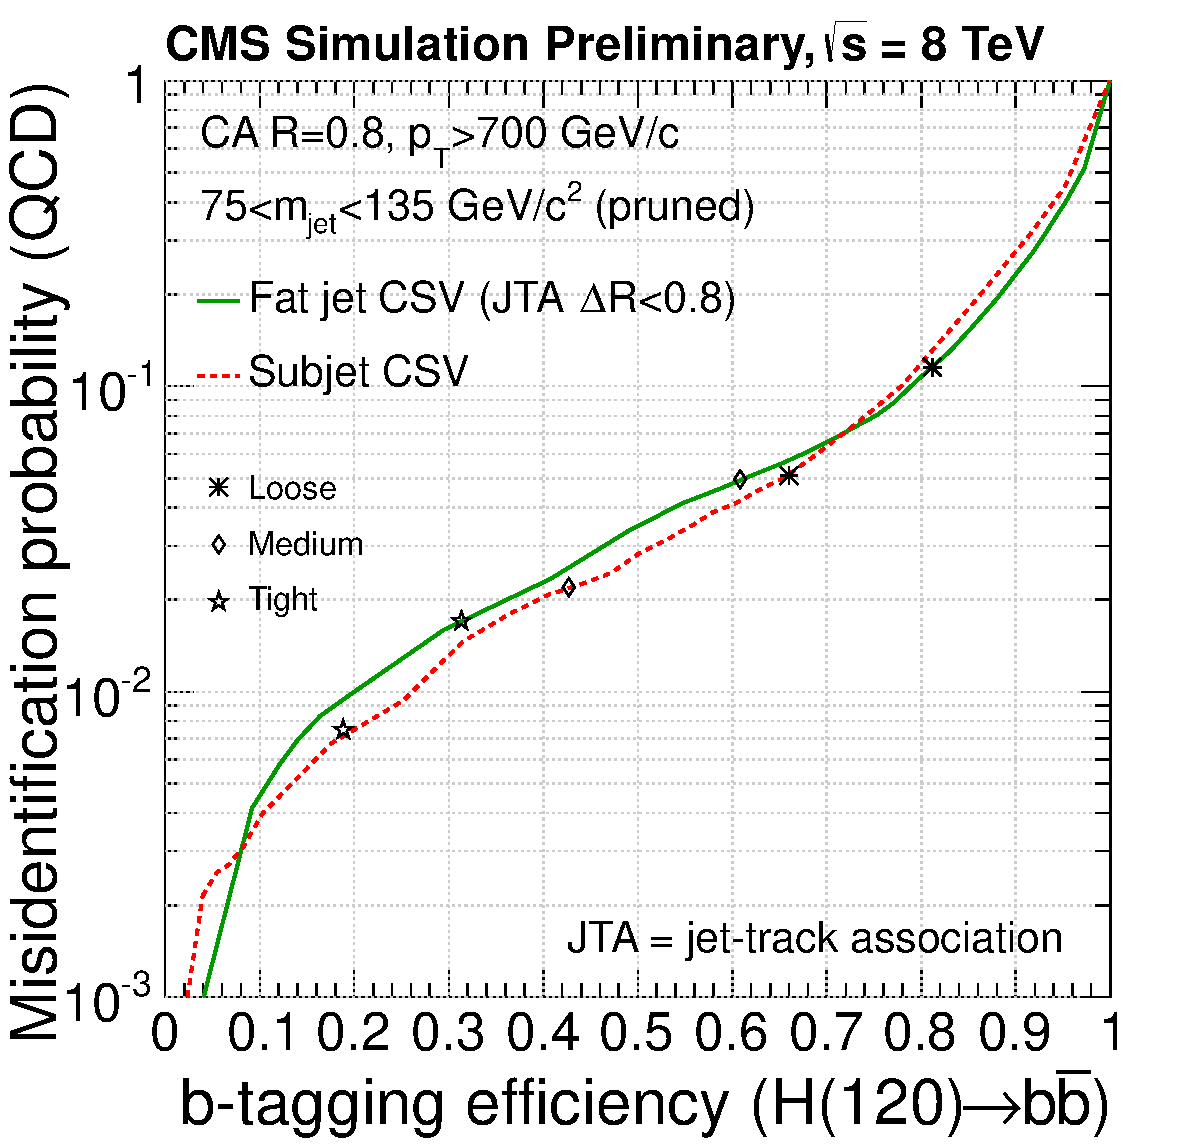
\includegraphics[width=0.45\textwidth]{\chseven/BTV-13-001_Figure_022-b.pdf}}
 \caption{Misidentification probability as a function of b tagging efficiency for boosted H $\to$ \bbbar jets and inclusive QCD jets for the CSV algorithm applied to large-cone jets
 and pruned subjets for large-cone jets with (a) 300 $< \pt < 500\GeV$ and (b) $\pt > 700\GeV$. Loose, medium, and tight operating points of the CSV discriminator are indicated~\cite{CMS:BTV13001}.}
\label{fig:htagging8TeV}
\end{figure}

The H tagging efficiency obtained combining the requirement on the pruned jet mass (75 $<$ \mJ $<$ 135\GeV)
and the subjet b tagging at the CSVL operating point is between 40 and 50\% for a H jet \pt range spanning from 300\GeV to 1\TeV,
with a suppression of QCD background to about 0.4\%.\\

The use of a fixed-size jet-track association cone inevitably leads to track sharing between the subjets of the jets once their angular separation becomes comparable
or smaller than the size of the association cone. 
For boosted H jets the fraction of shared tracks, defined as the ratio of the number of tracks within $\Delta R < 0.3$
from more than one subjet and the number of all tracks within $\Delta R < 0.3$ from any of the subjets,
ranges from a few percent at a jet \pt of 400\GeV
and increases to 40\% at a jet \pt of 700\GeV and to 80\% at a jet \pt of 1\TeV.
Figure~\ref{fig:subjetdR} shows the distribution of the angular separation $\Delta R$ of the two subjets reconstructed within the fat jet for different jet \pt ranges 
in simulated events of highly boosted Higgs bosons decaying to \bbbar.
Because of track sharing, the b tagging probabilities for individual subjets deteriorate at large jet \pt and the subjet b tagging performance approach the
fat jet b tagging ones as can be seen in Fig.~\ref{fig:htagging8TeV}.
The lost in efficiency is then recovered applying the two approaches depending on the $\Delta R$ between the two subjets.
In particular, the analysis involving boosted Higgs bosons such as the one presented in this work
apply subjet b tagging and fat jet b tagging if $\Delta R > 0.3$ and $< 0.3$, respectively. 

In the \lnuHjet analysis presented in this work a requirement on the pruned jet mass of the reconstructed H jet candidate given by 110 $<$ \mJ $<$ 135\GeV is used. The \mJ window is chosen such that a contamination from possible signals with boosted V jets in the Higgs boson mass region is minimized. The b tagging is performed with the algorithm described above using the loose working point of the CSV discriminant. The total H tagging efficiency for these selections is about 35\% for jet \pt of about 1 TeV with a mistagging probability below 1\%.

\begin{figure}[!htb]
 \begin{center}
  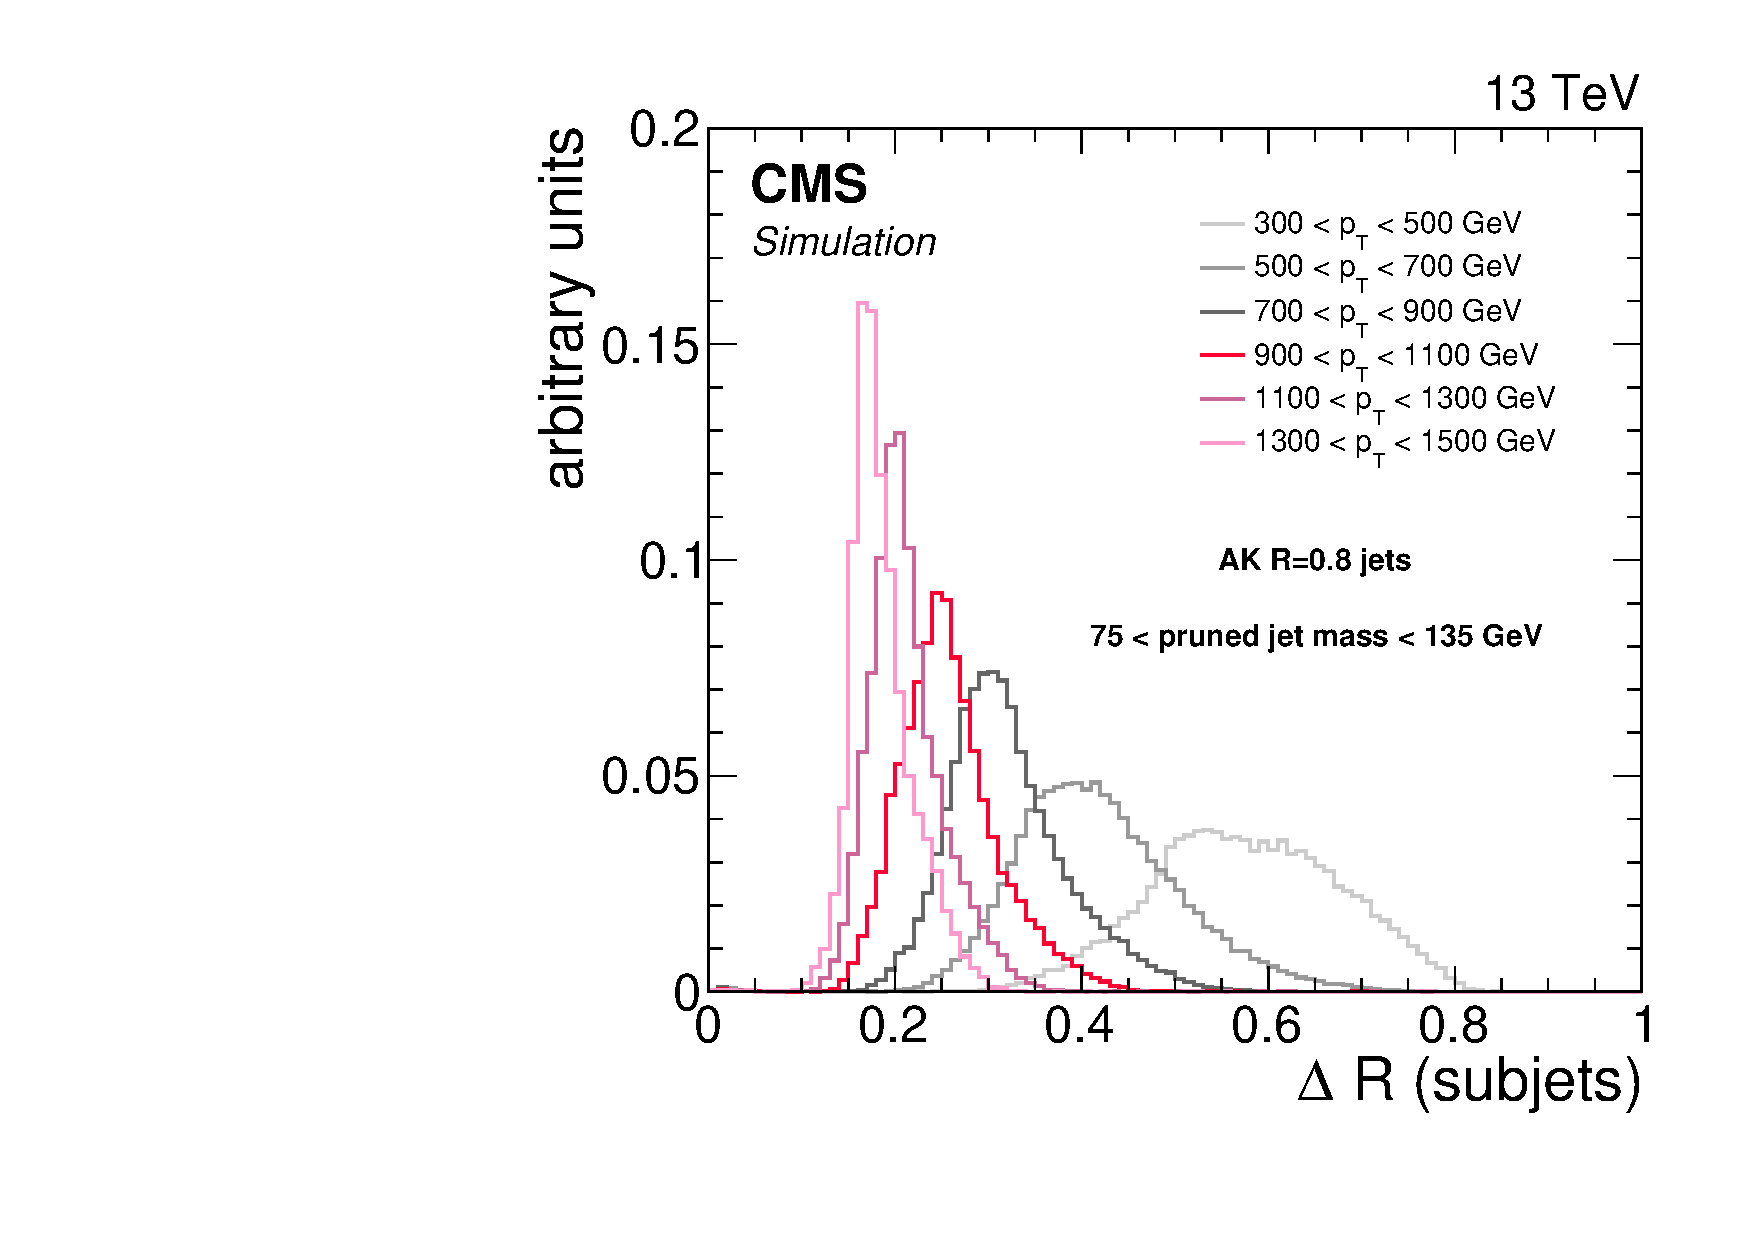
\includegraphics[width=0.5\textwidth]{\chseven/subjets-dr-vs-pt.pdf}
 \end{center}
 \caption{\small Distributions of the angular separation $\Delta R$ of the two subjets reconstructed within the fat jet for simulated events of highly boosted Higgs bosons decaying to \bbbar. The distributions are compared for different ranges of the H jet \pt.}
 \label{fig:subjetdR}
\end{figure}

%about the validation
The validation of b tagging in boosted H jets is performed selecting events containing jets from gluon splitting to \bbbar (g $\to$ \bbbar) in which the b quarks hadronize inside one large-cone jet~\cite{CMS:BTV13001}.
To enrich a sample of fat jets in g $\to$ \bbbar component, used as an analogue of boosted H $\to$ \bbbar jets, the fat jets are required to be double-muon-tagged with both subjets
matched to distinct muon candidates within a cone of size $\Delta R < 0.4$.
%Event samples containing high-\pt jets reconstructed using the CA8 algorithm are used to select such gluon splitting to \bbbar jets. The CA8 jets are required to have a transverse momentum \pt > 400 \GeV/.  The jet-pruning algorithm is used to decompose the fat jets into their subjet components. In order to enrich this sample in heavy-flavour jets, at least one of the two subjets can be required to be muon-tagged where a muon candidate with pT > 5 \GeV/ needs to be matched to a subjet within DR <0.4.  Finally, to additionally enrich a sample of fat jets in gluon splitting to bb component (g!bb), used as an analogue of boosted H!bb jets, the fat jets can be required to be double-muon-tagged with both subjets matched to distinct muon candidates. Furthermore, the validation of b tagging in boosted Higgs jets requires the presence of a jet with two b quarks within it.  One such standard model process consists of jets from gluon splitting to bb in which the two b quarks hadronise inside one jet.  Event samples containing high-pt jets reconstructed using the CA8 algorithm are used to select such gluon splitting to bb jets. The CA8 jets are required to have a transverse momentum \pt > 400 \GeV/.  The jet-pruning algorithm is used to decompose the fat jets into their subjet components. To remove infrared unsafe pruned subjet configurations, the following requirement is imposed [27]: DR(subjets)>Rcut2m/pT. Here DR (subjets) is the angular separation between the two subjets of a pruned CA8 jet, Rcut(=0.5) is the jet-pruning parameter, m the mass of the unpruned CA8 jet and pTis its transverse momentum.  This cut removes fat jets containing one very soft subjet with the other subjet nearly collinear with the fat jet axis. The selection described so far defines what is referred to as the inclusive sample of fat jets.  In order to enrich this sample in heavy-flavour jets, at least one of the two subjets can be required to be muon-tagged where a muon candidate with pT > 5 \GeV/ needs to be matched to a subjet within DR <0.4.  Finally, to additionally enrich a sample of fat jets in gluon splitting to bb component (g!bb), used as an analogue of boosted H!bb jets, the fat jets can be required to be double-muon-tagged with both subjets matched to distinct muon candidates. CA8 fat jets are labeled as b jets from gluon splitting (g!bb) if at least two generator-level b hadrons are found within DR<0.8 from the jet axis. However, for subjets of fat jets only the standard three flavour categories (udsg, c, and b) are used.
This sample is used to study the modelling of b tagging efficiencies in boosted H $\to$ \bbbar topologies.
The scale factors, given by the ratio between the efficiencies measured in data and simulation, are
found to be in good agreement with those measured in the standard, non-boosted topologies,
indicating that the simulation reproduces the b tagging performance in boosted and non-boosted enviroments equally well.
These scale factors are used in the analysis to reweight the simulated events.
%Overall, the scale factors measured in boosted topologies are found to be in good agreement
%with those measured in the standard, non-boosted topologies. This confirms observations from
%studies with boosted top jets, which indicate that the simulation reproduces the b tagging per-
%formance in boosted and non-boosted event topologies equally well.
%Dedicated studies using suitably defined control samples have been performed
%to validate the agreement of the data with the simulation and to measure the performance of
%b tagging in boosted environments.  A good agreement is found between measurements per-
%formed in boosted topologies with those performed in the standard, non-boosted topologies.

%%%%%%%%%%%%%%%%%%%%%%%%%%%%%%%%%%%%%%%%%%%%%%%%%%%%%%%%%%%%%%%%%%%%%%%%%%%